\documentclass[a5paper,9pt]{scrreprt}

%% Zeichensatz:
\usepackage[T1]{fontenc}	% Zeichensatz T1 verwenden
%% Zeichenkodierung:
\usepackage[utf8x]{inputenc}	% Unicode-Transformation-Format
%% Schriftsatz:
\usepackage{default}
\usepackage{times}
\usepackage[babel,german=swiss]{csquotes} % Schweizer Anführungszeichen
\usepackage{amsmath} 		% AMS mathematics
\usepackage{amssymb} 		% AMS symbols

%% Silbentrennung, etc.
\usepackage{ngerman}		% Deutsch nach neuer Rechtschreibung
\usepackage[ngerman]{babel}	% Deutsch nach neuer Rechtschreibung

%% Formatierung
\usepackage{graphicx} 		% zum Einbinden von Bildern (GIF, PNG und JPEG)
\usepackage{color} 		% farben ...
% \usepackage{pdfpages} 	% zum Einbinden von pdf-Dateien
\usepackage{calc,layouts,multicol}
\usepackage{geometry}
\usepackage{blindtext,microtype}
\usepackage{textcomp}
\usepackage{booktabs}
\usepackage{array}		% zur Benutzung von Tabellen

%% Verlinkungen im Dokument
% \usepackage[setpagesize,bookmarks,bookmarksopen]{hyperref}

%% Quellcode
\usepackage{listings}						% Quellcode als Text einbinden
\lstset{language=Python}

%% Bibliografie 
\bibliographystyle{gerplain}

%% Titelei
\author{Bruggmann Roland}
\subject{Schwerpunktfach Physik und Angewandte Mathematik}
\title{Numerische Methoden\\Approximation und Integration\\Programmierung TI-89}
\date{Luzern, Mai 2005}
\medskip 
\publishers{Maturit\"atsschule f\"ur Erwachsene MSE, Reussb\"uhl}

\begin{document}
\maketitle[-1] % Argument: Seitennummer f\"ur die Erste Seite der Titelei

\begin{abstract}
Diese Arbeit dokumentiert eine Implementierung numerischer Methoden zur Approximation (Bisection, Regula falsi, Newton) und Integration (Rechteck-, Trapez-, Tangenten-, Simpson-Verfahren) f\"ur den Taschenrechner TI-89.

Als Programmiersprache kommt TI-BASIC zum Einsatz, den Quellcode zum Programm \enquote{nummeth() -- Numerische Methoden} habe ich auf einer Intel-x86-Maschine mit GNU/Linux als Betriebssystem und dem Editor \enquote{Kate} erstellt. Um das Programm auf den TI-89 zu laden, verwendete ich die Software \enquote{TiLP}.

Als Nachschlagwerke und Grundlage zur Programmierung dienten mir ausschliesslich das dem TI-89 von Texas Instruments mitgelieferte Benutzerhandbuch zur Advanced Mathematics Software Version 2.0 \cite{AVM99} in gedruckter Form sowie die Hinweise zur Version 2.8 \cite{AVM02} als PDF.
\end{abstract}

\setcounter{secnumdepth}{2}
\tableofcontents

\chapter{Bemerkungen zu Beginn}
\section{Allgemeines}
Kenntnisse zur Bedienung des TI-89 werden voraussgesetzt und k\"onnen z.B. im zum Rechner mitgelieferten Benutzerhandbuch \cite{AVM99} nachgeschlagen werden.

Im Programm \verb|nummeth| kann mit \verb|ESC| jeweils zum vorherigen Fenster gewechselt werden. Numerische Eingaben werden jeweils auf ihre G\"ultigkeit gepr\"uft. Bei einer ung\"ultigen Eingabe erscheint eine Fehlermeldung. Danach besteht die M\"oglichkeit, die Eingabe zu korrigieren.

\section{Erfassen von Funktionen}
\subsection*{Vor dem Programmstart}
Funktionen k\"onnen im \verb|Y-Editor| eingegeben und im Bildschirm \verb|Graph| zur Wahl des Intervalls untersucht werden.

Die im \verb|Y-Editor| eingegebenen Funktionen \verb|y1(x)| bis \verb|y10(x)| stehen dem Programm \verb|nummeth| zur Verf\"ugung, k\"onnen darin also optional ausgew\"ahlt werden -- sowohl bei einer Approximation als auch bei einer Inte­gration.

\subsection*{Nach dem Programmstart}
Eine Funktion kann auch erst nach dem Programmstart mit den anderen Parametern (Intervall, Iterationen etc.) erfasst werden (siehe folgende Kapitel sowie das Flussdiagramm im Anhang \ref{sec:Flowchart}).

\chapter{Das Programm}
\section{Programm starten}
Mit dem Start des Programms werden einige Konfigurationen ausgel\"ost: Das Programm wird auf Fehler \"uberpr\"uft, aktuelles Ver­zeich­nis wird nach M\"oglichkeit \verb|NUMERIK|, aktuelle Einstellungen der Modi unter \verb|MODE| werden gesichert und f\"ur die Dauer des Pro­gramm­ab­laufs konfiguriert, eine Parameterliste wird erstellt und der \verb|Y-Editor| wird auf erfasste Funk­tio­nen untersucht. Dies kann beim erst­ma­ligen Gebrauch des Programms einige Sekunden dauern.

\subsection*{Start mit VAR-LINK}
Mit \verb|2nd| $\blacktriangleright$ \verb|VAR-LINK| kann der Variablen-Bildschirm aufgerufen werden. Im Folder \verb|NUMERIK| ist die Pro­gramm­variable \verb|nummeth| zu finden (siehe Abbildung \ref{fig:VARLINK}). Diese ist mit dem Cursor zu markieren und mit der Taste \verb|ENTER| zu bes­t\"a­ti­gen.
\begin{figure}[h]
  \centering
  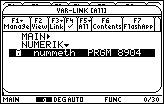
\includegraphics[width=4cm]{img/nummeth_image001.png}
  \caption{Variablen-Ordner}
  \label{fig:VARLINK}
\end{figure}

\newpage
Der Pfad der Programmvariablen ist somit in die Eingabezeile kopiert worden. Dieser muss nun noch mit einer schliessenden runden Klammer '\verb|)|' erg\"anzt werden (siehe Abbildung \ref{fig:CLI}). Mit \verb|ENTER| wird das Programm gestartet.
\begin{figure}[h]
  \centering
  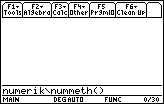
\includegraphics[width=4cm]{img/nummeth_image003.png}
  \caption{Eingabezeile mit kopiertem Pfad}
  \label{fig:CLI}
\end{figure}

\subsection*{Start mit CATALOG}
Mit \verb|CATALOG| $\blacktriangleright$ \verb|F4 User-Defined| werden gespeicherte Funk­tions- und Programmvariablen an­ge­zeigt. Mit dem Cursor den Pfeil zu \verb|nummeth(| bewegen (siehe Abbildung \ref{fig:CATALOG}) und die Taste \verb|ENTER| bet\"atigen.

Der Pfad der Programmvariablen ist somit in die Eingabezeile kopiert worden. Dieser muss nun noch mit einer schliessenden runden Klammer '\verb|)|' erg\"anzt werden (siehe Abbildung \ref{fig:CLI}). Mit \verb|ENTER| wird das Programm gestartet.
\begin{figure}[h]
  \centering
  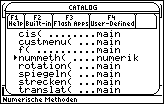
\includegraphics[width=4cm]{img/nummeth_image005.png}
  \caption{Variablen-Katalog}
  \label{fig:CATALOG}
\end{figure}

\newpage
\section{Aufgabe, Methode, Parameter f(x) (optional)}
\subsection*{Aufgabe}
Die Wahl der Aufgabe erfolgt per Cursor im Drop-Down-Menu, best\"atigen mit \verb|ENTER| (siehe Abbildung \ref{fig:Aufgabe}).
\begin{figure}[h]
  \centering
  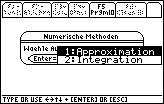
\includegraphics[width=4cm]{img/nummeth_image008.png}
  \caption{Dialog 'Numerische Methoden: Aufgabe’}
  \label{fig:Aufgabe}
\end{figure}

% \newpage
\subsection*{Methode}
Die Wahl der Methode erfolgt per Cursor im Drop-Down-Menu, best\"atigen mit \verb|ENTER| (siehe Abbildung \ref{fig:MethodeApproximation}).
% (siehe Abbildungen \ref{fig:MethodeApproximation} und \ref{fig:MethodeIntegration}).
\begin{figure}[h]
  \centering
  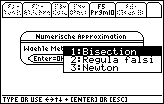
\includegraphics[width=4cm]{img/nummeth_image010.png}
  \caption{Dialog 'Numerische Approximation: Methode’}
  \label{fig:MethodeApproximation}
\end{figure}
% \begin{figure}[h]
%   \centering
%   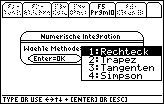
\includegraphics[width=4cm]{img/nummeth_image012.png}
%   \caption{Dialog 'Numerische Integration: Methode’}
%   \label{fig:MethodeIntegration}
% \end{figure}

\newpage
\subsection*{Parameter f(x)}
Sind im \verb|Y-Editor| Funktionen erfasst worden, erscheint nach der Wahl einer Methode ein Dialog 'Parameter’ mit der M\"oglichkeit, eine der erfassten Funktionen zur weiteren Bearbeitung auszuw\"ahlen. Dies erfolgt im Drop-Down-Menu 'Funktion aus dem Y-Editor uebernehmen?’ durch die Wahl des Eintrages 'Ja’ (siehe Abbildung \ref{fig:ParameterFxFrage}).
\begin{figure}[h]
  \centering
  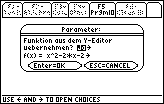
\includegraphics[width=4cm]{img/nummeth_image014.png}
  \caption{Dialog 'Parameter: Funktion aus dem Y-Editor uebernehmen?'}
  \label{fig:ParameterFxFrage}
\end{figure}

Die Wahl der Funktion erfolgt per Cursor im Drop-Down-Menu 'f(x) = ’ (siehe Abbildung \ref{fig:ParameterFxWahl}). Hat eine der erfassten Funktionen mehr als 18 Zeichen, wird die Variable der Funktion angezeigt (z.B. \verb|y3(x) ; analog der Bezeichnung im \verb|Y-Editor ).
\begin{figure}[h]
  \centering
  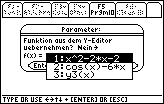
\includegraphics[width=4cm]{img/nummeth_image016.png}
  \caption{Dialog 'Parameter: f(x) = '}
  \label{fig:ParameterFxWahl}
\end{figure}

\newpage
\section{Erfassen der Parameter}
Der Wechsel zwischen dem Eingabemodus f\"ur Ziffern und jenem f\"ur Buchstaben dient die alpha-Taste. In folgenden Dialogen kann eine Funktion f(x) erfasst werden, falls nicht schon im \verb|Y-Editor| eingegeben.

\subsection{Approximation}
\subsubsection*{Bisection oder Regula falsi}
Zu beachten: F\"ur diese Methoden muss das Intervall so gew\"ahlt werden, dass der Funktions­wert f(a) kleiner, der Funktions­wert f(b) gr\"osser ist als Null. Der Wert f\"ur 'n Iterationen' muss eine ganze, positive Zahl sein.
\begin{figure}[h]
  \centering
  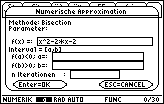
\includegraphics[width=4cm]{img/nummeth_image018.png}
  \caption{Dialog 'Numerische Approximation: Methode Bisection'}
  \label{fig:ParameterApproximationBisection}
\end{figure}
\begin{figure}[h]
  \centering
  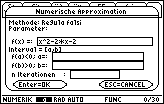
\includegraphics[width=4cm]{img/nummeth_image020.png}
  \caption{Dialog 'Numerische Approximation: Methode Regula falsi'}
  \label{fig:ParameterApproximationRegulaFalsi}
\end{figure}

\newpage
\subsubsection*{Newton}
Der Startwert f\"ur die Methode Newton muss wie folgt gew\"ahlt werden:
\begin{itemize}
  \item Der Funktionswert darf nicht Null betragen (d.h. f(startwert) ≠ 0).
  \item Die Steigung der Tangente durch den Startwert darf nicht Null sein (d.h. f’(startwert) ≠ 0).
\end{itemize}
F\"ur die Methode nach Newton kann zwischen der Anzahl Iterationen und der Genauigkeit gew\"ahlt werden.
\begin{itemize}
  \item n Iterationen: Die Berechnung wird nach n Iterationen ab­ge­bro­chen.
  \item Genauigkeit eps: Die Berechnung wird abgebrochen, sobald der Betrag der Differenz der letzten zwei Resultate kleiner als der in eps angegebene Wert ist.
\end{itemize}
\begin{figure}[h]
  \centering
  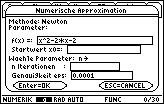
\includegraphics[width=4cm]{img/nummeth_image022.png}
  \caption{Dialog 'Numerische Approximation: Methode Newton'}
  \label{fig:ParameterApproximationNewton}
\end{figure}

\newpage
\subsection{Integration}
Zu beachten: F\"ur diese Methoden muss das Intervall so gew\"ahlt werden, dass die Funktions­werte f(a) und f(b) gr\"osser als Null sind, wobei b > a ist. Der Wert f\"ur 'n Schritte' muss eine ganze, positive Zahl sein.

\subsubsection*{Rechteck- oder Trapez-Verfahren}
\begin{figure}[h]
  \centering
  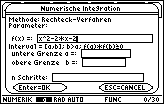
\includegraphics[width=4cm]{img/nummeth_image024.png}
  \caption{Dialog 'Numerische Integration: Methode Rechteck-Verfahren'}
  \label{fig:ParameterIntegrationRechteck}
\end{figure}
\begin{figure}[h]
  \centering
  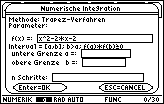
\includegraphics[width=4cm]{img/nummeth_image026.png}
  \caption{Dialog 'Numerische Integration: Methode Trapez-Verfahren'}
  \label{fig:ParameterIntegrationTrapez}
\end{figure}

\newpage
\subsubsection*{Tangenten- oder Simpson-Verfahren}
Zu beachten: Bei diesen Methoden muss der Wert f\"ur die Variable n gerade sein.
\begin{figure}[h]
  \centering
  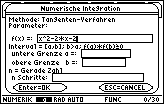
\includegraphics[width=4cm]{img/nummeth_image028.png}
  \caption{Dialog 'Numerische Integration: Methode Tangenten-Verfahren'}
  \label{fig:ParameterIntegrationTangente}
\end{figure}
\begin{figure}[h]
  \centering
  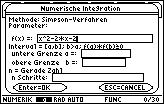
\includegraphics[width=4cm]{img/nummeth_image030.png}
  \caption{Dialog 'Numerische Integration: Methode Simpson-Verfahren'}
  \label{fig:ParameterIntegrationSimpson}
\end{figure}

\newpage
\section{Resultate speichern}
\subsection{Variablenname}
Um die errechneten Resultate zu speichern, werden Variablennamen wie folgt generiert:
\begin{itemize}
    \item Matrizenvariable f\"ur die Ergebnisse:
    \begin{itemize}
      \item die ersten drei Buchstaben der Aufgabe (\textbf{App}roximation oder \textbf{Int}egration)
      \item die ersten vier Buchstaben der Methode (Approximation: \textbf{Bise}ction, \textbf{Regu}la falsi oder \textbf{Newt}on; Integration: \textbf{Rech}teck, \textbf{Trap}ez, \textbf{Tang}enten oder \textbf{Simp}son)
      \item die Ziffer \textbf{1} als m\"oglicher Z\"ahler
      \item Beispiele: \textbf{AppRegu1}, \textbf{IntTang1}
    \end{itemize}
    \item Variable f\"ur die Nullstellen:
    \begin{itemize}
      \item \textbf{NS} als Kurzform f\"ur \textbf{N}ull\textbf{s}telle
      \item die ersten vier Buchstaben der Methode (\textbf{Bise}ction, \textbf{Regu}la falsi, \textbf{Newt}on)
      \item die Ziffer \textbf{1} als m\"oglicher Z\"ahler
      \item Beispiele: \textbf{NSBise1}, \textbf{NSNewt1}
    \end{itemize}
\end{itemize}
Diese Variablennamen k\"onnen selbstverst\"andlich ge\"andert werden. Zu beachten: Die Variablennamen-L\"ange ist im TI-89 auf acht Zeichen beschr\"ankt.

Existiert im Verzeichnis Numerik bereits eine Variable mit gew\"ahltem Variablennamen, wird dies mit dem Dialog 'Matirzenvariable' gemeldet (siehe Abbildung \ref{fig:Matirzenvariable}). Mit \verb|ENTER| wird die bestehende Variable \"uberschrieben, mit \verb|ESC| kann zur\"uck in die Resultat-Anzeige gewechselt und die Variable editiert werden.
\begin{figure}[h]
  \centering
  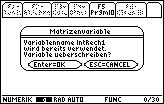
\includegraphics[width=4cm]{img/nummeth_image032.png}
  \caption{Dialog 'Matirzenvariable'}
  \label{fig:Matirzenvariable}
\end{figure}

\newpage
\subsection{Approximation}
Nullstelle sowie Ergebnisse k\"onnen im Dialog 'Resultat’ ins angegebene Verzeichnis gespeichert werden (siehe Abbildung \ref{fig:ResultatApproximationBisection}).
% (siehe Abbildungen \ref{fig:ResultatApproximationBisection}, \ref{fig:ResultatApproximationRegulaFalsi} und \ref{fig:ResultatApproximationNewton}).
\begin{figure}[h]
  \centering
  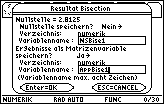
\includegraphics[width=4cm]{img/nummeth_image034.png}
%   \caption{Dialog 'Resultat Bisection’}
  \caption{Dialog 'Resultat’ f\"ur die Methode Bisection}
  \label{fig:ResultatApproximationBisection}
\end{figure}
% \begin{figure}[h]
%   \centering
%   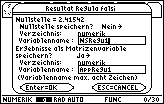
\includegraphics[width=4cm]{img/nummeth_image036.png}
%   \caption{Dialog 'Resultat Regula falsi’}
%   \label{fig:ResultatApproximationRegulaFalsi}
% \end{figure}
% \begin{figure}[h]
%   \centering
%   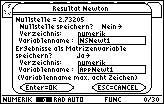
\includegraphics[width=4cm]{img/nummeth_image038.png}
%   \caption{Dialog 'Resultat Newton’}
%   \label{fig:ResultatApproximationNewton}
% \end{figure}

% \newpage
\subsection{Integration}
Die Ergebnisse k\"onnen per Dialog 'Resultat’ ins angegebene Verzeichnis gespeichert werden (siehe Abbildung \ref{fig:ResultatIntegrationRechteck}).
% (siehe Abbildungen \ref{fig:ResultatIntegrationRechteck}, \ref{fig:ResultatIntegrationTrapez}, \ref{fig:ResultatIntegrationTangente} und \ref{fig:ResultatIntegrationSimpson}).
\begin{figure}[h]
  \centering
  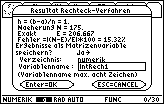
\includegraphics[width=4cm]{img/nummeth_image040.png}
%   \caption{Dialog 'Resultat Rechteck-Verfahren’}
  \caption{Dialog 'Resultat' f\"ur die Methode Rechteck-Verfahren}
  \label{fig:ResultatIntegrationRechteck}
\end{figure}
% \begin{figure}[h]
%   \centering
%   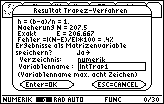
\includegraphics[width=4cm]{img/nummeth_image042.png}
%   \caption{Dialog 'Resultat Trapez-Verfahren’}
%   \label{fig:ResultatIntegrationTrapez}
% \end{figure}
% \begin{figure}[h]
%   \centering
%   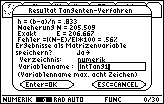
\includegraphics[width=4cm]{img/nummeth_image044.png}
%   \caption{Dialog 'Resultat Tangenten-Verfahren’}
%   \label{fig:ResultatIntegrationTangente}
% \end{figure}
% \begin{figure}[h]
%   \centering
%   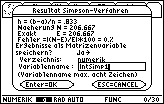
\includegraphics[width=4cm]{img/nummeth_image046.png}
%   \caption{Dialog 'Resultat Simpson-Verfahren’}
%   \label{fig:ResultatIntegrationSimpson}
% \end{figure}

\newpage
\section{Ende der Berechnungen}
\begin{figure}[h]
  \centering
  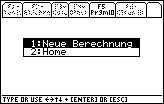
\includegraphics[width=4cm]{img/nummeth_image048.png}
  \caption{Pop-Up 'Neue Berechnung’}
  \label{fig:NeueBerechnung}
\end{figure}
\begin{itemize}
  \item Neue Berechnung: Die Routine kehrt zur\"uck zur Auswahl der Aufgabe.
  \item Home: Der Bildschirm \verb|Home| wird eingeblendet, aktuelles Verzeichnis wird das aktuelle Verzeichnis vor Programmstart, \verb|MODE|-Einstellungen werden zur\"uckgesetzt auf den Stand wie vor dem Programmstart.
  \item Achtung: \verb|ESC| sollte hier nicht verwendet werden, da sonst ein m\"oglicher Fehler (Undefined Variable) das Zur\"uckstellen der \verb|MODE| -Einstellungen auf die zu Beginn gesicherten Parameter umgeht.
\end{itemize}

\chapter{Resultate als Matrizenvariable}
Die als Matrizenvariable gespeicherten Resultate k\"onnen mit \verb|APPS| $\blacktriangleright$ \verb|6:Data/Matrix| \verb|Editor| $\blacktriangleright$ \verb|2:Open...| ge\"offnet werden (siehe Abbildung \ref{fig:Applications}). Folgende Eintr\"age in den Drop-Down-Menus m\"ussen gew\"ahlt werden (siehe Abbildung \ref{fig:Open}):
\begin{itemize}
  \item Als 'Type' muss 'Matrix' gew\"ahlt werden.
  \item 'Folder' ist das Verzeichnis, in das die Matrize gespeichert wurde.
  \item 'Variable' ist der Name der Matirzenvariable.
\end{itemize}
\begin{figure}[h]
  \centering
  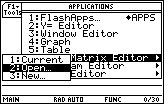
\includegraphics[width=4cm]{img/nummeth_image050.png}
  \caption{Applikationen}
  \label{fig:Applications}
\end{figure}
\begin{figure}[h]
  \centering
  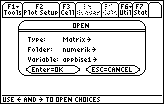
\includegraphics[width=4cm]{img/nummeth_image052.png}
  \caption{\"Offnen-Dialog}
  \label{fig:Open}
\end{figure}
In die Matrize werden jeweils auch Aufgabe, Methode und Funktion gespeichert, damit ersichtliche ist, wie die Resultate zustande kamen. In der Tabelle kann mit den Pfeiltasten gearbeitet werden: Der Inhalt der aktiven Zelle wird jeweils in der Eingabezeile eingeblendet (siehe Abbildung \ref{fig:Matrix}).
\begin{figure}[h]
  \centering
  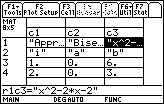
\includegraphics[width=4cm]{img/nummeth_image054.png}
  \caption{Resultate als Matrize}
  \label{fig:Matrix}
\end{figure}


\listoffigures

\bibliography{./bib/nummeth}

\appendix
\chapter{Flussdiagramm}
\label{sec:Flowchart}
\begin{figure}[h]
  \centering
  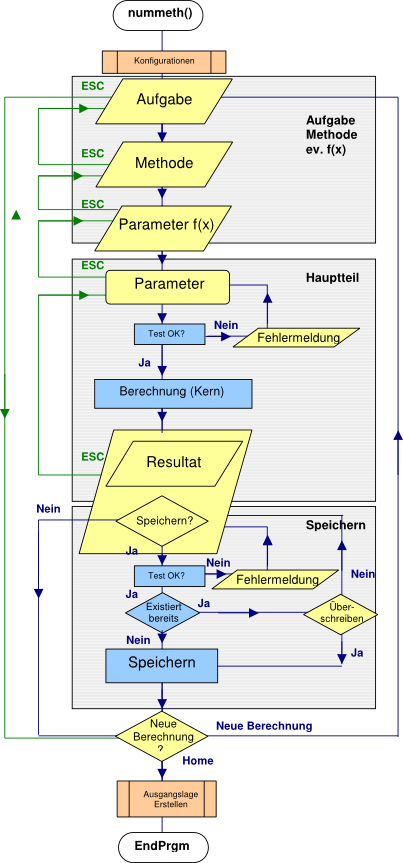
\includegraphics[height=0.74\textheight]{img/nummeth_flowchart.png}
%   \caption{Flussdiagramm zu nummeth}
%   \label{fig:Flowchart}
\end{figure}

% \newpage
% \chapter{Quellcode}
% \begin{description}
%     \item[Autor:] Roland Bruggmann
%     \item[Date:] 29. April 2005
%     \item[Version:] 1.02
%     \item[Synopsis:] nummeth() is a program written in TI-BASIC for the pocket calculator TI-89 and serves with well known methods for numeric approximation and numeric integration.
\end{description}

% \begin{verbatim}
:nummeth()
:Prgm
:@Numerische Methoden 
    Numerische Approximation 
    (Bisection, Regula falsi, Newton) und 
    Numerische Integration 
    (Rechteck−, Trapez−, Tangenten−, Simpson−Verfahren)
    Hinweis: 
    y1 bis y10 des Y-Editors koennen 
    ins Programm uebernommen werden
:@ Version 1.02, 29. April 2005
:@ Roland Bruggmann
:@ Email: roland.bruggmann@gmx.net
:ClrIO
:Disp ""
:Disp "..."
:@Konfigurationen
:Local i,oldfoldr,yeditor,z,gmlist
:@Verzeichnis
:getFold()→oldfoldr
:Lbl neuverz
:Try
:  setFold(numerik)
:Else
:  ClrErr
:  Try
:    NewFold numerik
:  Else
:    ClrErr
:    Goto modus
:  EndTry
:  Goto neuverz
:EndTry
:@Modus
:Lbl modus
:getMode("0")→gmlist
:setMode({
	  "1","1",
	  "3","1",
	  "4","1",
	  "5","1",
	  "6","1",
	  "7","1",
	  "8","1",
	  "12","1",
	  "13","1",
	  "14","1"})
:@Parameterliste
:Try
:  dim(numlist)
:Else
:  ClrErr
:  {"","","",""}→numlist
:EndTry
:@Y−Editor:y1 bis y10
:DelVar x
:0→z
:For i,1,10
:  expr("y"&string(i)&"(x)")→yeditor
:  If string(yeditor)≠"y"&string(i)&"(x)" Then
:    1+z→z
:    If dim(string(yeditor))>18 Then
:      "y"&string(i)&"(x)"→ylist[z]
:    Else
:      string(yeditor)→ylist[z]
:    EndIf
:  EndIf
:EndFor
:Try
:  dim(ylist)
:Else
:  ClrErr
:  {"no"}→ylist
:EndTry
:@Aufgabe,Methode,Parameter1
:Local auf,meth,msf,msn,msm,mspa,msw,
  pml,auflist,m1list,m2list
:"f(x) ="→msf
:"Numerische "→msn
:"Methode: "→msm
:"Parameter:"→mspa
:"Waehle "→msw
:{"Approximation","Integration"}→auflist
:{"Bisection","Regula falsi","Newton"}→m1list
:{"Rechteck","Trapez","Tangenten","Simpson"}→m2list
:{"Ja","Nein"}→qlist
:Lbl aufgabe
:Dialog
:  Title msn&"Methoden"
:  DropDown msw&"Aufgabe:",auflist,auf
:EndDlog
:If ok=0
:  Goto neub
:Lbl methode
:Dialog
:  Title msn&auflist[auf]
:  DropDown msw&msm,expr("m"&string(auf)&"list"),meth
:EndDlog
:If ok=0
:  Goto aufgabe
:Lbl pam1
:If ylist[1]≠"no" Then
:  2→pml
:  Dialog
:    Title mspa
:    Text "Funktion aus dem Y-Editor"
:    DropDown "uebernehmen?",qlist,pml
:    DropDown msf,ylist,yl
:  EndDlog
:  If ok=0
:    Goto methode
:  If pml=1
:    ylist[yl]→numlist[1]
:EndIf
:@Hauptteil
:Local a,b,k,msfa,msi,msnt,n,titl,w
:" failed"→msfa
:"Interval = [a,b]"→msi
:" isn't true"→msnt
:Lbl anfang
:If auf=2 Then
:  @Integration
:  Local h,s,msger,msv,ms21,ms22
:  "-Verfahren"→msv
:  "b>a"→ms21
:  "f(a)*f(b)≥0"→ms22
:  numlist[1]→fstring
:  numlist[2]→n
:  numlist[3]→a
:  numlist[4]→b
:  If meth>2 Then
:    "n = Gerade Zahl "→msger
:  Else
:    ""→msger
:  EndIf
:  @Parameter
:  Dialog
:    Title msn&auflist[auf]
:    Text msm&m2list[meth]&msv
:    Text mspa
:    Text ""
:    Request msf,fstring,0
:    Text msi&"; "&ms21&"; "&ms22
:    Request "untere Grenze a =",a
:    Request "obere Grenze
:    b =",b
:    Text msger
:    Request "n Schritte",n
:  EndDlog
:  If ok=0 Then
:    If ylist[1]="no"
:    Goto methode
:    Goto pam1
:  EndIf
:  {fstring,n,a,b}→numlist
:  For i,1,dim(numlist)
:    If numlist[i]=""
:      Goto anfang
:  EndFor
:  @Test n=gerade
:  If meth>2 and remain(expr(n),2)>0 Then
:    Text msger&msnt
:    Goto anfang
:  EndIf
:  @Test Interval
:  expr(fstring)→f(x)
:  expr(a)→a
:  expr(b)→b
:  For i,1,2
:    If not expr(#("ms2"&string(i))) Then
:      Text expr("ms2"&string(i))&msnt
:      Goto anfang
:    EndIf
:  EndFor
:  @Kern
:  expr(n)→n
:  (b-a)/n→h
:  If meth<3 Then
:    @Kern rechteck u. trapez
:    f(a)/meth→s
:    setMode({"14","3"})
:    [[0,a,f(a),s,h*s]]→loesung
:    For i,1,n-1
:      a+i*h→w
:      s+f(w)→s
:      augment(loesung;[[i,w,f(w),s,h*s]])→loesung
:    EndFor
:    If meth=2 Then
:      @trapez
:      s+f(b)/2→s
:      augment(loesung;[[n,b,f(b),s,h*s]])→loesung
:    EndIf
:    h*s→res
:  ElseIf meth=3 Then
:    @Kern tangenten
:    a+h→w
:    f(w)→s
:    setMode({"14","3"})
:    [[1,w,f(w),s,2*h*s]]→loesung
:    For i,3,n-1,2
:      a+i*h→w
:      s+f(w)→s
:      augment(loesung;[[i,w,f(w),s,2*h*s]])→loesung
:    EndFor
:    2*h*s→res
:  ElseIf meth=4 Then
:    @Kern simpson
:    f(a)→s
:    2→k
:    setMode({"14","3"})
:    [[0,a,f(a),s,h/3*s]]→loesung
:    For i,1,n-1
:      6-k→k
:      a+i*h→w
:      s+k*f(w)→s
:      augment(loesung;[[i,w,f(w),s,h/3*s]])→loesung
:    EndFor
:    s+f(b)→s
:    augment(loesung;[[n,b,f(b),s,h/3*s]])→loesung
:    h/3*s→res
:  EndIf
:  @Exakt,Fehler,Titelmatrize
:  Local exakt,fehler
:  Try
:    string(approx(∫(f(x),x,a,b)))→exakt
:  Else
:    ClrErr
:    msfa→exakt
:    msfa→fehler
:    Goto titel
:  EndTry
:  string(approx(round(abs((res-expr(exakt))
      /(expr(exakt)))*100,2)))&"%"→fehler
:  Lbl titel
:  setMode({"14","1"})
:  [[auflist[auf]&";"&expr("m"&string(auf)&"list")[meth]&msv,
      fstring,
      "h="&string(approx(h)),
      "Exakt="&exakt,
      "Fehler="&fehler]
      ["i","xi","f(xi)","ε","ΣA"]]→titl
:Else
:  @Approximation
:  Local msit,stel
:  "n Iterationen     "→msit
:  If meth=3 Then
:    @Newton
:    Local bed,bed1,bed2,eps,ms13,pa,palist,x0,x1
:    "Startwert "→ms13
:    {"n","eps"}→palist
:    numlist[1]→fstring
:    numlist[2]→n
:    "0.0001"→eps
:    numlist[4]→x0
:    @Parameter
:    Dialog
:      Title msn&auflist[auf]
:      Text msm&m1list[meth]
:      Text mspa
:      Text ""
:      Request msf,fstring,0
:      Request ms13&"x0=",x0
:      DropDown msw&mspa,palist,pa
:      Request msit,n
:      Request "Genauigkeit eps",eps
:    EndDlog
:    If ok=0 Then
:      If ylist[1]="no"
:        Goto methode
:      Goto pam1
:    EndIf
:    {fstring,n,eps,x0}→numlist
:    If fstring="" or numlist[pa+1]="" or x0=""
:      Goto anfang
:    @Test Startwert
:    expr(fstring)→f(x)
:    expr(x0)→x0
:    d(f(x),x)→g(x)
:    If f(x0)*g(x0)=0 Then
:      Text ms13&msfa&": f(x0)*f'(x0)=0"
:      Goto anfang
:    EndIf
:    @Kern Newton
:    expr(n)→n
:    expr(eps)→eps
:    "i=n"→bed1
:    "abs(x1-x0)<eps"→bed2
:    expr("bed"&string(pa))→bed
:    [[auflist[auf],expr("m"&string(auf)&"list")[meth],
      fstring,""]
      ["i","xi","f(xi)","f'(xi)"]]→titl
:    setMode({"14","3"})
:    [[0,x0,f(x0),g(x0)]]→loesung
:    1→i
:    Loop
:      x0-f(x0)/(g(x0))→x1
:      augment(loesung;[[i,x1,f(x1),g(x1)]])→loesung
:      If expr(bed)
:        Exit
:      x1→x0
:      i+1→i
:    EndLoop
:    setMode({"14","1"})
:    If pa=1 Then
:      7→stel
:    Else
:      dim(string(fPart(eps)))+1→stel
:    EndIf
:    x1→res
:  Else
:    @Bisection/Regula falsi
:    Local kern,kern1,kern2,ms11,ms12
:    "f(a)<0"→ms11
:    "f(b)>0"→ms12
:    numlist[1]→fstring
:    numlist[2]→n
:    numlist[3]→a
:    numlist[4]→b
:    @Parameter
:    Dialog
:      Title msn&auflist[auf]
:      Text msm&m1list[meth]
:      Text mspa
:      Text ""
:      Request msf,fstring,0
:      Text msi
:      Request ms11&"; a=",a
:      Request ms12&"; b=",b
:      Request msit,n
:    EndDlog
:    If ok=0 Then
:      If ylist[1]="no"
:        Goto methode
:      Goto pam1
:    EndIf
:    {fstring,n,a,b}→numlist
:    For i,1,dim(numlist)
:      If numlist[i]=""
:        Goto anfang
:    EndFor
:    @Test Interval
:    expr(fstring)→f(x)
:    expr(a)→a
:    expr(b)→b
:    For i,1,2
:      If not expr(#("ms1"&string(i))) Then
:        Text expr("ms1"&string(i))&msnt
:        Goto anfang
:      EndIf
:    EndFor
:    @Kern Bisection/Regula falsi
:    expr(n)→n
:    @Formel bisection
:    "(a+b)/2"→kern1
:    @Formel regula-falsi
:    "a-(b-a)/(f(b)-f(a))*f(a)"→kern2
:    expr("kern"&string(meth))→kern
:    [[auflist[auf],expr("m"&string(auf)&"list")[meth],
      fstring,"",""]
      ["i","a","b","xi","f(xi)"]]→titl
:    expr(kern)→w
:    setMode({"14","3"})
:    [[1,a,b,w,f(w)]]→loesung
:    For i,2,n
:      If f(w)<0 Then
:        w→a
:      Else
:        w→b
:      EndIf
:      expr(kern)→w
:      augment(loesung;[[i,a,b,w,f(w)]])→loesung
:    EndFor
:    7→stel
:    w→res
:  EndIf
:  setMode({"14","1"})
:EndIf
:augment(titl;loesung)→loesung
:@Hauptteil Ende
:@Resultat
:Local msa,mse,msma,msns,msr,mssp,msvn,msvz,
    fldr,namelist,reslist,splist,varlist,ma,ns
:getFold()→fldr
:"max. acht Zeichen)"→msa
:"Ergebnisse als "→mse
:"Matrizenvariable "→msma
:"Nullstelle "→msns
:"Resultat "→msr
:"speichern? "→mssp
:"Variablenname "→msvn
:" Verzeichnis:"→msvz
:left(auflist[auf],3)
    &left(expr("m"&string(auf)&"list")[meth],4)
    &"1"→name1
:2→ns
:Lbl resultat
:If auf=1 Then
:  @Approximation
:  "NS"&left(m1list[meth],4)&"1"→name2
:  Dialog
:    Title msr&m1list[meth]
:    Text msns&"= "&string(round(res,stel))
:    DropDown " "&msns&mssp,qlist,ns
:    Text msvz&fldr
:    Request msvn,name2
:    Text mse&msma
:    DropDown mssp&" ",qlist,ma
:    Text msvz&fldr
:    Request msvn,name1
:    Text " ("&msvn&msa
:  EndDlog
:Else
:  @Integration
:  ""→name2
:  Dialog
:    Title msr&m2list[meth]&msv
:    Text " h = (b-a)/n = "&string(round(h,3))
:    Text " Naeherung N = "&string(round(res,6))
:    Text " Exakt
:    E = "&exakt
:    Text " Fehler =|(N-E)/E|*100 = "&fehler
:    Text mse&msma
:    DropDown mssp&" ",qlist,ma
:    Text msvz&fldr
:    Request msvn,name1
:    Text " ("&msvn&msa
:  EndDlog
:EndIf
:If ok=0
:  Goto anfang
:{ma,ns}→splist
:If splist={2,2}
:  Goto neub
:@Test Variablennamen
:{name1,name2}→namelist
:For i,1,2
:  If splist[i]=1 and (namelist[i]="" or dim(namelist[i])>8)
:    Goto resultat
:EndFor
:If splist[2]=1 and namelist[2]="x" Then
:  Dialog
:    Title msns
:    Text msvn&"x unzulaessig"
:  EndDlog
:  If ok=0
:    Goto resultat
:  Goto resultat
:EndIf
:@Speichern
:{msma,msns}→varlist
:0→z
:For i,1,2
:  Lbl neuname
:  If z=1 Then
:    Dialog
:      Title varlist[i]
:      Text msvn&namelist[i]
:      Text "wird bereits verwendet."
:      Text "Variable ueberschreiben?"
:    EndDlog
:    If ok=0
:      Goto resultat
:    DelVar #(expr("name"&string(i)))
:    0→z
:  EndIf
:  If i=1 and splist[1]=1 Then
:    Try
:      @Matirzenvariable
:      Rename loesung,#name1
:    Else
:      If errornum=270 Then
:        ClrErr
:        1→z
:        Goto neuname
:      Else
:        PassErr
:      EndIf
:    EndTry
:  ElseIf i=2 and splist[2]=1 Then
:    Try
:      @Nullstelle
:      Rename res,#name2
:    Else
:      If errornum=270 Then
:        ClrErr
:        1→z
:        Goto neuname
:      Else
:        PassErr
:      EndIf
:    EndTry
:  EndIf
:EndFor
:@Neue Berechnung?
:Lbl neub
:Local nb
:PopUp {"Neue Berechnung","Home"},nb
:If nb=1 Then
:  Goto aufgabe
:ElseIf nb=2 Then
:  DispHome
:EndIf
:@Ausgangslage erstellen
:DelVar fstring,f,g,loesung,name1,name2,res,yl,qlist,ylist
:setMode(gmlist)
:Try
:  setFold(#oldfoldr)
:Else
:  ClrErr
:EndTry
:EndPrgm
\end{verbatim} 

\end{document}
